\chapter{The State of the Resarch}
\label{chap:results}

\section{Tissue Models}
The skin absorbs majority of incident \gls{rf} \gls{em} energy, and the power penetration depth is below about \SI{8}{\mm} and well below \SI{1}{\mm} at \SI{6}{\GHz} and \SI{30}{\GHz}, respectively.
Therefore, from the \gls{em} dosimetry point of view, tissue models should consist only of skin but a detailed knowledge of the internal skin structure is necessary to produce accurate predictions of \gls{rf} energy into tissue~\cite{Ziskin2018Tissue}.
On the other hand, from the thermal dosimetry point of view, it is necessary to include deeper tissues as well because the resulting surface temperature rise is determined by the thermal resistance of subcutaneous tissues even though the bulk of the \gls{em} energy is absorbed right at and slightly below the sole surface of the skin~\cite{Ziskin2018Tissue}.
As thermal modeling is out of the scope of this work, focus is put only on the tissue models for the \gls{em} dosimetry above \SI{6}{\GHz}. 

The details description of the structure of the skin, together with variations given age, sex and race, is outlined in~\cite{Snyder1979Report}.
The skin consists of two major layers -- the epidermis and dermis.
The epidermis is composed of five layers: the stratum corneum, stratum lucidum, stratum granulosum, stratum spinosum, and stratum basale.
Since the epidermis has no blood supply, but has a constant water content across all sub-layers (except stratum corneum which is water-free), it can be treated as the same layer when absorption of \gls{rf} energy is considered at and above \SI{6}{\GHz}.
The dermis consists of two layers: the papillary and reticular layer.
Additionally, the hypodermis, which is adipose tissue, lies beneath the dermis and has a much lower water content compared to the dermis.
Since fat has a low heat transfer coefficient, in this configuration, the overall upper skin layer acts as the thermal barrier.

Most of exposure assessment and/or computational dosimetry studies for local exposure above \SI{6}{\GHz} use planar tissue-equivalent single-, e.g.,~\cite{Nakae2020Skin,Poljak2020Assessment,Ziane2020Antenna}, or multi-layer models, e.g.,~\cite{Wu2015Safe,Foster2018Modeling,He2018RF}.
In the case of single-layer stratified models, typically the dielectric parameters of ``dry skin'' are considered and no detailed thermal anlysis is provided.
In the case of multi-layer models, either three or four distinct layers are considered as follows: the epidermis, dermis, hypodermis, and in some instances, muscle layer.
Dielectric properties are most often extracted by using the five-term Cole-Cole model~\cite{Gabriel1996Compilation}.  

\section{Spatial Averaging Considerations}
It is stated in the \gls{icnirp} guidelines~\cite{ICNIRP2020Guidelines} and the \gls{ieee} standard~\cite{IEEE2019Standard} that a square averaging area of \SI{4}{\cm\squared} provides a close approximation to maximum temperature rise due to \gls{rf} heating above \SI{6}{\GHz}.
This resolution is based mainly on thermal modeling study~\cite{Hashimoto2017On} where it is suggested that planar control surface for averaging with area of $2 \times 2$ \SI{}{\cm\squared}, shown in \cref{fig:averaging_surface}, is a good measure to correlate with the local peak temperature elevation when the field distribution is close to uniform within the area.
\begin{figure}[ht]
    \centering
    \begin{subfigure}[b]{0.51\textwidth}
        \centering
        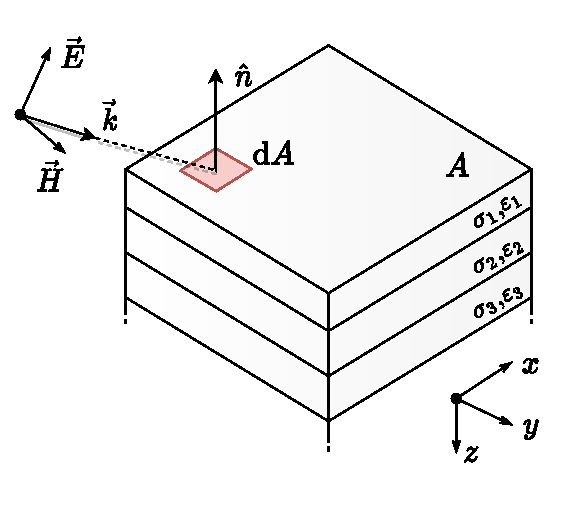
\includegraphics[width=\linewidth]{artwork/averaging_surface.a.pdf}
        \caption{3-D point of view.}
        \label{fig:averaging_surface_a}
    \end{subfigure}
    \begin{subfigure}[b]{0.42\textwidth}
        \centering
        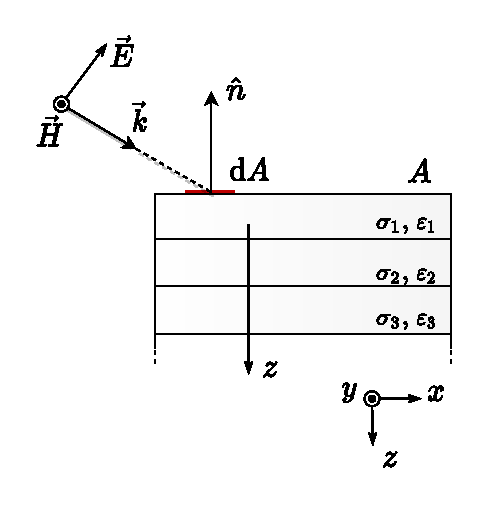
\includegraphics[width=\linewidth]{artwork/averaging_surface.b.pdf}
        \caption{Lateral point of view.}
        \label{fig:averaging_surface_b}
        \end{subfigure}
    
    \caption{Control surface for averaging on the multi-layer tissue-equivalent block model.}
    \label{fig:averaging_surface}
\end{figure}
The results from the study are based on the heating factor -- a ratio between the power density averaged on the area and maximum temperature rise on the same area, by considering a multi-layer tissue model exposed to three different sources of \gls{em} fields -- plane wave, a dipole antenna, and an antenna array.
The area of \SI{4}{\cm\squared} achieves consistency with the volume-averaged dosimetric quantities below \SI{6}{\GHz} as the front facing surface of 10-g cubic volume is about the same area ($2.15 \times 2.15$ \SI{}{\cm\squared} assuming constant tissue density of \SI{1000}{\kg\per\m\cubed}).

At higher frequencies (generally above \SI{30}{\GHz} for most exposure scenarios), the area of \SI{4}{\cm\squared} is not suitable because of the non-uniformity of the field distribution within such a large surface.
Thus, it is proposed in~\cite{Hashimoto2017On}, considering the results from the analytical study~\cite{Foster2016Thermal}, that the power density should be averaged on the most exposed area of \SI{1}{\cm\squared} for exposure above \SI{30}{\GHz} to better capture extremely focused beams.
An additional criterion is further imposed -- the (maximum) power density averaged over square \SI{1}{\cm\squared} area must not exceed 2 times the value for the corresponding averaging area of \SI{4}{\cm\squared}.

As the power density distribution, either incident or absorbed, on the front facing surface of the exposed tissue is computed numerically, it is of utmost importance to choose an appropriate averaging technique.
According to~\cite{Foster2022Three}, the \gls{fdtd} method was introduced to computational dosimetry and bioelectromagnetics in general in 1987 by Gandhi~\cite{Sullivan1987Use} as it was shown to be well adapted to \gls{em} computations at \gls{rf} frequencies.
Currently, the \gls{fdtd} method is the standard method in numerical dosimetry owing mostly to the advent of well-polished commercial software~\cite{Hirata2021Human}.
However, to achieve high-fidelity values of power density on the surface of conformal tissue-equivalent body models, especially at \gls{5g} frequencies, including \gls{mmw}, it is necessary to use methods that employ a structural instead of a grid-like spatial domain discretiztaion.
More details on this subject are available elsewhere, e.g., in~\cite{Poljak2018On}.
In cases of regular grid, the surface is computationally reconstructed implicitly via cubical cells.
The spatial averaging is then crudely approximated as the averaged sum of contributions on each cell.
On the other hand, in cases of structural mesh, the surface is reconstructed by using the structural mesh composed of 2-D simplices for which there is a large array of corresponding efficient and accurate quadrature schemes, e.g., for disks~\cite{Kim1997Symemetric}, triangles~\cite{Dunavant1985High} and quadrilaterals~\cite{Dunavant1985Economical}.
The spatial averaging is then approximated by actually solving the surface integral of either the scalar (the first definition of the \gls{apd}, $S_\text{ab, 1}$, outlined in \cref{eqn:apd_1} and the norm definition of the \gls{ipd}, $S_\text{inc, tot}$, given in \cref{eqn:ipd-magnitude}) or vector field by using a 2-D quadrature technique of choice (the second definition of the \gls{apd}, $S_\text{ab, 2}$, outlined in \cref{eqn:apd_1} and the normal definition of the \gls{ipd}, $S_\text{inc, n}$, given in \cref{eqn:ipd-normal}).

\section{Local Exposure Assessment and Dosimetry Literature Review}
The current state of the literature is reviewed based upon the available studies accessible through the EMF-portal platform -- an internet information platform of the RWTH Aachen University which systematically summarizes scientific research data on the effects of \gls{em} fields on human body.
The core of the EMF-Portal is the literature database with 37,436 publications and 6,979 summaries of individual scientific studies\footnote{The total number of papers in the database was read on 2022, December 23rd at: \url{https://www.emf-portal.org/en}.}.

The following query was used to extract relevant studies:
\begin{verbatim}
    (power OR "power density")
    AND (average OR averaged OR area OR spatially)
    AND year=x
    AND (topic=technical_dosimetric
         OR topic=law_recommendation_guideline
         OR topic=review_survey_summary)
    AND (frequencyRange=radio_frequency
         OR frequencyRange=mobile_communications)
\end{verbatim}
where keywords are either ``power'' or ``power density'' together with either ``average'', ``averaged'', ``area'' or ``spatially''.
Keywords such as ``incident'', ``transmitted'', ``absorbed'' or even ``epithelial'' have been deliberately omitted in order to include both exposure assessment and computational dosimetry studies in the consideration regardless of authors' preference of terminology.
Additionally, the selected topics are technical dosimetry studies, laws, recommendation documents or guidleines associated with the aforementioned keywords, and review studies.
Finally, in the above query, the selected frequency range includes all bands that are classified within \gls{rf} and mobile communications ($f \geq \SI{10}{\MHz}$).
However, the purpose of this document is to review only the studies that pertain to spatial averaging of power density on the surface of the exposed tissue above \SI{6}{\GHz}.
Thus, additionally, only the studies which refer to the \SIrange[range-units=single,range-phrase=--]{6}{300}{\GHz} range are extracted manually.
This extraction was done per publication year of each research paper, from 1998 -- the year of publication of the previous version of the \gls{icnirp} guidelines~\cite{ICNIRP2020Guidelines}, ending with 2022 -- the year when this document was written.
A special emphasis is placed on the most recent studies, written after 2019 and 2020, when a new dosimetric quantity by means of the \gls{apd} was introduced in international exposure limits, and which is used for limiting local exposure to \gls{em} fields at the \SIrange[range-units=single,range-phrase=--]{6}{300}{\GHz} range.

\subsubsection*{1998 -- 2007}
During the 1998 to 2007 period, only a few of published studies addressed the spatial averaging of the power density on an exposed control surface, with only two studies considered exposure above \SI{6}{\GHz}.
This can be attributed to the fact that most wireless communication systems fell into the higher \SI{}{\MHz} range --  the \gls{em} power penetration depth is significant, thus \gls{sar} was considered a relevant dosimetric quantity.

However, limits to approximate exposure above \SI{10}{\GHz} in the far-field zone were given in terms of the \gls{ipd} spatially averaged on \SI{20}{\cm\squared} planar control surface in \gls{icnirp} 1998 guidelines~\cite{ICNIRP1998Guidlines}.
The \gls{ipd} was set to \SI{10}{\watt\per\meter\squared} and \SI{50}{\watt\per\meter\squared} for general public and occupational exposure, respectively.
Furthermore, local exposure was quantified by the spatially-averaged \gls{ipd} over the most exposed region of \SI{1}{\cm\squared} and was limited to \SI{200}{\watt\per\meter\squared} and \SI{1000}{\watt\per\meter\squared} for general public and occupational exposure, respectively.

In the \gls{ieee} standard published in 1999~\cite{IEEE1999Standard}, recommendations have been stated to prevent any potential adverse health effect by \gls{rf} \gls{em} fields and are intended to apply to exposures in both controlled (occupational exposure) and uncontrolled environments (general public).
Maximum permissible exposure is defined in terms of either the \gls{rms} electric and magnetic field strength, equivalent plane-wave power densities measured in free space, and currents induced within the human body to which a person may be exposed without adverse health effects and with an acceptable safety factor.
Above \SI{6}{\GHz}, the maximum permissible exposure in terms of the spatially-averaged power density for local body parts is set to a constant value of \SI{100}{\watt\per\meter} for occupational exposure, while it is defined as a function of frequency ($f / 150$) up to \SI{15}{\GHz}, but again set to a constant value of \SI{100}{\watt\per\meter} above \SI{15}{\GHz} for general public.
These values have been derived upon the \gls{br}s given by means of the stead-state volume-averaged \gls{sar}.
Spatial averaging is defined as the \gls{rms} of the power density over an area equivalent to the vertical cross section of the human body (projected area) at a distance of at least \SI{20}{\cm} from any object.

Given the maximum permissible exposure as defined in the previous two exposure limits~\cite{IEEE1999Standard,ICNIRP1998Guidlines}, in~\cite{Hirata2000Temperature}, the authors investigate temperature rise in the human eye for plane wave exposures at \SIrange[range-units=single,range-phrase=--]{0.6}{6}{\GHz}.
The numerical results are obtained by solving the Pennes bioheat equation~\cite{Pennes1948Analysis} with forcing term given by means of \gls{sar} given the specific frequency of impinging \gls{em} fields.
Maximum temperature rise due to the \gls{ipd} of \SI{50}{\watt\per\meter\squared} is \SI{0.3}{\celsius} at \SI{6}{\GHz}.
The value of the \gls{ipd} is chosen to match the maximum permissible exposure limit for occupational exposure as per~\cite{Ulcek1997Evaluating}.
In this document, spatial averaging is performed by taking the mean value of the power density over an area approximately equivalent to the vertical cross-section (projected area) of the exposed part of the human body.

In human study~\cite{Walters2000Heating}, thermal pain thresholds were measured in 10 subjects during brief exposure at \SI{94}{\GHz} with the \gls{ipd} set to extremely high value of \SI{18}{\kW\per\meter\squared}.
It is found that the pain threshold for pricking pain is \SI{43.9}{} $\pm$ \SI{0.7}{\celsius} (\SI{95}{\percent} confidence interval, which corresponds to the maximum surface temperature rise of about \SI{9.9}{\celsius}.
The results are in a very good agreement with the simple 1-D analytical model based on the Pennes bioheat equation~\cite{Pennes1948Analysis}.
In this study, the \gls{ipd} is spatially averaged over the planar projection of the human back in 2-D.
For purposes of specifying the \gls{ipd}, the spatial averaging is performed simply by computing the mean power density within the most exposed region (where \SI{90}{\percent} of the total incident power density was distributed).

Finally, in~\cite{Faraone2000Estimation}, a set of analytical formulas has been postulated to estimate the averaged power density in the close proximity of base-station collinear array antennas.
Authors suggest that the \gls{ipd} averaged over the whole body can be used to verify compliance to maximum permissible exposure limits for antenna-to-body separation distances larger than $\lambda/2$ where there is no significant coupling between the antenna and body and where electrical properties of the antenna are constant during exposure.
Further, under the assumption of the cylindrical character of \gls{em} fields in the immediate vicinity of the array, the average power density is given as:
\begin{align}
    \bar{P}_\text{d}(\rho) \approx \frac{P_\text{rad}}{2L \cdot 2\pi\rho},
\end{align}
where
\begin{align}
    P_\text{rad} \approx 2\pi\rho \int_{-L}^{L} \Re \Big( \frac{1}{2} \; E_z \; H_\Phi^* \Big),
\end{align}
and where $P_\text{rad}$ represents the power radiated by the collinear array of half-wavelength dipole antennas with $2N +1$ radiating elements, each excited by a time-harmonic current, $I_n$.
Other parameters are as follows: $2L$ is the overall length of the antenna with each element separated from each other by the distance $p \leq \lambda$, $\rho$ is the distance away from the antenna, $E_z$ and $H_\Phi$ are the amplitude of the $z$-component of the electric and the $\Phi$-component of the magnetic field, respectively.
With an increase in distance from the antenna, the above quantity undergoes transition from the cylindrical decay in the near field, to the spherical in the far field (details available in subsection B of section II in~\cite{Faraone2000Estimation}).
The main contribution of this paper is the outlined set of formulas for the accurate prediction of the average exposure from different sources, from collinear arrays to other directive antennas.
These formulas can be adjusted to take into account the partial exposure as:
\begin{align}
    \bar{P}_\text{d}(\rho, L; T, H) \approx P_\text{d}(\rho, L) \cdot \frac{T}{H}, \quad \rho << G_A \; L,
\end{align}
where $G_A$ stands for the collinear array broadside gain, and where $T$ and $H$ represent the height of the person standing parallel in front of the antenna and $t$ is the intercepted portion.
The advantage of using the concept of average power density as presented in this work is the simplicity of evaluation of the exposure of humans near cellular base-station antennas, but unfortunately it does not take into account an actual local exposure and predicts only a single-point measure of the worst-case \gls{ipd}.

In the revised version of the \gls{ieee} 1999 standard~\cite{IEEE1999Standard}, it was prescribed that the exposure limit for general public given by means of the spatially-averaged \gls{ipd} is \SI{10}{\W\per\m\squared} at \SIrange[range-units=single,range-phrase=--]{3}{10}{\GHz} range.
The power density should be spatially averaged over any contiguous area corresponding to $100 \lambda^2$.
In addition, maximum spatial peak power densities of $18.56 \cdot f_G^{0.699}$
and \SI{200}{\watt\per\m\squared} were defined at the \SIrange[range-units=single,range-phrase=--]{3}{30}{\GHz} 
and above \SI{30}{\GHz}, respectively, where $f_G$ is the frequency of the impinging \gls{em} field in \SI{}{\GHz}.
However, no averaging area or spatial sampling density was officially specified to assess the spatial peak power density limits.

\subsubsection*{2008 -- 2017}
In two studies published by the same research group, the question of what is the appropriate exposure metric at the \SIrange[range-units=single,range-phrase=--]{1}{10}{\GHz} range -- \gls{sar} or \gls{ipd}, is discussed by using the simple 1-D planar model~\cite{Anderson2010SAR} and complex human body models~\cite{McIntosh2010SAR}.

In the first study~\cite{Anderson2010SAR}, the most appropriate transition frequency at which the \gls{ipd} should replace volume-averaged \gls{sar} as the \gls{br} is discussed.
It is based on Monte Carlo analysis with varying input parameters such as tissue thicknesses and body sites.
The results show that the peak \gls{sar} is better indicator of maximum surface temperature rise across the entire examined spectrum compared to the \gls{ipd}.
Furthermore, peak 10-g \gls{sar} achieves only marginally better predictive power than its 1-g counterpart.
As the tissue is represented by using the 1-D multi-layer model, no spatial averaging is conducted to evaluate the \gls{ipd}, which is addressed in the subsequent study~\cite{McIntosh2010SAR}.

Instead of 1-D planar tissue models, in~\cite{McIntosh2010SAR}, complex human body models, i.e., heterogeneous head models of an adult and a 12-year-old, for a variety of exposure scenarios have been utilized to assess the frequency at which the transition in \gls{br} -- from \gls{sar} to \gls{ipd}, is appropriate.
Numerical results show that the maximum temperature rise on the surface correlate better with the peak 10-g \gls{sar} up to \SI{6}{\GHz} compared to the \gls{ipd}.
On the contrary to the previous analytical study~\cite{Anderson2010SAR}, above \SI{6}{\GHz}, the results show significantly better correlation of the \gls{ipd} with maximum temperature rise.
Considering combined conclusions from both studies, authors suggest that the transition frequency should be set to \SI{6}{\GHz}.

Discussion on the transition frequency is conducted in~\cite{Colombi2015} where the implication of this transition is further addressed by means of the the maximum possible radiated power from a device used in close proximity to the human body.
The results of this study have demonstrated the non-physical discontinuity in the maximum radiated power as the transition is made from \gls{sar} to the \gls{ipd}.
This means that devices should use significantly lower radiated power (in order of several \SI{}{\decibel}) to achieve compliance above \SI{6}{\GHz}.
Two key observations of this study are as follows: (i) the necessity of the harmonization of the transition frequency for \gls{br}s across all internationally defined exposure limits by standardization organizations and regulatory authorities, and (ii) averaging areas in~\cite{ICNIRP1998Guidlines,IEEE2005Standard} are not appropriate and lead to inconsistency in defining exposure above the transition frequency.

Similar conclusions have been outlined in~\cite{Thors2016Exposure} where complex numerical simulations of exposure to array antennas in \gls{5g} mobile communication equipment have been conducted.
Here, a systematic study varying parameters such as the frequency, array size, array topology, antenna-to-body separation distance, and beam steering range is considered and compared to the measured data.
Overall conclusion is that a global harmonization of the exposure limits above \SI{6}{\GHz} is necessary to avoid unjustified decrease of the maximum transmitted power of \gls{5g} user equipment compared to preceding generations.
The spatial averaging of the power density in this paper is conducted as defined in \cref{eqn:ipd-normal}.

Furthermore, as a sequel to results presented in~\cite{Colombi2015,Thors2016Exposure}, in~\cite{Xu2017Understanding}, the difference between definitions of the maximum spatially-averaged power density and the influence of different interpretations on the maximum permissible transmitted power of user equipment mock-ups employing a patch array operating at \SI{15}{\GHz} have beem presented.
First interpretation is taken from~\cite{Thors2016Exposure} where \gls{ipd} is spatially averaged on the square shaped control surface by following the formulation given in \cref{eqn:ipd-normal}.
Surface integral of the vector field is approximated to obtain the total power flux density that passes through the averaging area and subsequently normalized with that area.
The second interpretation is the maximum arithmetic mean value of the power density over the averaging area, analogous to \cref{eqn:ipd-magnitude}.
The main difference is that in the first interpretation only the normal components of the power density vector are considered, whereas in the second definition tangential components are included.
In the reactive near-field zone, there is always an antenna-body coupling present due to the reflected \gls{em} power density flowing back inwards user equipment, it is thus reasonable to expect that the second interpretation will yield results that are greater than the values obtained by the first interpretation of the spatially-averaged \gls{ipd}.
Numerical results demonstrate the overall dependence of the difference of maximum permissible transmitted power to comply with the \gls{icnirp} 1998 guidelines~\cite{ICNIRP1998Guidlines} are \SIrange[range-units=single,range-phrase=--]{1}{2.6}{\decibel} depending on the antenna-to-body separation distance.
Authors here again appeal that all regulatory organizations should not only agree upon the transition frequency but also to explicitly state the definition of the maximum spatially-averaged \gls{ipd} to remove any exiting ambiguities.

Finally, the research outlined so far culminates in the publication of the seminal work~\cite{Hashimoto2017On} where the authors discuss both the averaging area for the \gls{ipd} and the transition frequency.
The relationship between the size of the area over which incident power density is averaged and the local peak temperature elevation in a tissue-equivalent multi-layer model by means of the heating factor has been reported.
This relationship is based on the numerical data obtained by simulating exposure of the model to different radiating sources (plane-wave, half-wavelength dipole, and dipole array) at the \SIrange[range-units=single,range-phrase=--]{3}{300}{\GHz} range.
It has been shown that over \SI{70}{\percent} of the absorbed power is located within the boundaries of the \SI{4}{\cm\squared} region on the most exposed surface which mostly determines maximum surface temperature increase.
Thus, an averaging area of $2 \times 2$ \SI{}{\cm\squared} provides a good measure to correlate with local peak temperature rise when the field distribution is nearly uniform across that area.
Additionally, above \SI{30}{\GHz}, the averaging should be performed on $1 \times 1$ \SI{}{\cm\squared} averaging surface to account for localized beam formation and to capture non-uniformities.
These findings have served exceptionally well for defining the revised version of the \gls{ieee} standard and \gls{icnirp} guidelines that followed in 2019 and 2020, respectively.

\subsubsection*{2018-present}
In~\cite{Christ2018Thermal}, the analysis of temperature rise on the surface of single- and multi-layer- tissue-equivalent models positioned in close proximity to generic \gls{5g} wireless devices with phased array antennas operating at \SI{28}{} and \SI{100}{\GHz} has been presented.
Temperature increase is quantified in relation to both the electric field amplitude to take into account the possible impact of reactive components of the incident field in the near-field zone, and the real part of the power density flux across \SI{20}{} and \SI{1}{\cm\squared} planar control area on the exposed surface of the model.
Authors argue that the size of the averaging area along with the layering structure of the tissue are two most important parameters for exposure assessment and temperature increase on the surface.
For an averaging area of \SI{1}{\cm\squared}, normalization of surface temperature rise to both the electric field and \gls{ipd} yield similar results, whereas an averaging area of \SI{20}{\cm\squared} shows differences depending on the normalization for the smaller antenna array at \SI{100}{\GHz}.
The overall conclusion is that the spatially-averaged\gls{ipd} represents an accurate proxy for temperature rise and can serve to assess compliance provided the averaging surface is appropriately defined with regard to the exposure scenario.
Finally, authors call for the urgent need of additional analysis to establish a robust correlation of the averaged power density values with the induced temperature increase as well as to establish the most suitable shape of the surface for averaging.

In line with~\cite{Hashimoto2017On}, in~\cite{Funahashi2018Averaging}, additional analysis of the \gls{ipd} spatially-averaged on the square surface of \SI{1}{} and \SI{4}{\cm\squared} at the \SIrange[range-units=single,range-phrase=--]{10}{100}{\GHz} range has been performed.
The correlation with maximum temperature rise on the exposed surface is examined for the case of patch antenna arrays with 4 by 1, 2 by 2, and 3 by 3 elements, and compared with 1-D analysis~\cite{Foster2017Thermal}.
It is confirmed that the \SI{4}{\cm\squared} averaging area is suitable up to \SI{30}{\GHz}, but the smaller averaging area is needed above \SI{30}{\GHz} because the non-uniform \gls{em} field distribution.
Additionally, this study finds that the square shaped averaging area of \SI{4}{\cm\squared}, characterized by the heat diffusion length, should be the most appropriate by means of the shape and size considering it corresponds to the face area of the \gls{sar} averaging 10-g volume under the assumption that the mass density is \SI{1000}{\kg\per\meter\cubed}~\cite{Hirata2019Setting}.
This leads to preserved consistency in the ratio of maximum temperature rise in the skin to the \gls{sar} averaged over \SI{10}{\g} of tissue, which is confirmed to be a valid metric to assess compliance~\cite{Hirata2003Temperature,Hirata2009correlation,McIntosh2010SAR}.

Authors of the same group as in~\cite{Funahashi2018Averaging} performed computations of the area-averaged \gls{tpd} at the skin as a new potential metric to estimate the steady-state skin temperature elevation above the transition frequency.
The results were obtained at \SIrange[range-units=single,range-phrase=--]{3}{300}{\GHz} for the case of multi-layer homogeneous cube with dielectric and thermal properties of the skin and additionally compared to the realistic human body model.
Numerical results have shown excellent agreement with 1-D analytical solution first presented in~\cite{Foster2017Thermal} and confirm the area-averaged \gls{tpd} as a potential surrogate of surface temperature rise.
The averaging area of \SI{4}{\cm\squared} again have been shown as appropriate for frequencies up to \SI{300}{\GHz} provided that they are supplemented by limits on the intensity of very small beams.
If not, the reduction of an averaging area by a factor of 4 for small beamwidths should be a reasonable choice, and provides continuity with far-infrared guidelines $ > \SI{300}{\GHz}$.
A large contribution of this study is the introduction of a new metric of the power density that is no longer measured in free space but rather represents the internal/dosimetric quantity for estimating surface temperature above transition frequency.
During the time of writing~\cite{Funahashi2018Averaging}, this metric was discussed and mentioned in the \gls{icnirp} public consultation document and \gls{ieee} C95.1 draft for the 2019 version of the \gls{ieee} standard~\cite{IEEE2019Standard}.
Mathematically, it is identical to \cref{eqn:tpd} and, once averaged, should correspond to \cref{eqn:apd_1} which is currently the official \gls{br} above \SI{6}{\GHz} in both the \gls{ieee} C95.1-2019 standard~\cite{IEEE2019Standard} and \gls{icnirp} 2020 guidelines~\cite{ICNIRP2020Guidelines} for limiting local steady-state exposure.
Unfortunately, the spatial averaging in this work is not explicitly outlined.
It is stated, however, that the spatially-averaged \gls{tpd} is approximated by multiplying a transmission coefficient by the \gls{ipd}, which is obtained beforehand as the magnitude of the Poynting vector in free space averaged over an area of either \SI{4}{} or \SI{1}{\cm\squared} (in square shape), depending on frequency, on the plane where the model surface exists.

Two studies~\cite{He2018RF,Miura2021Power} have performed \gls{rf} compliance analysis of surface temperature elevation in human head model at \SI{28}{\GHz} realistic sources, e.g., beam-steering patch arrays, dipoles, etc., which was the expected frequency for the \gls{5g} commercial products.
In~\cite{He2018RF}, authors confirm that the power density averaged over \SI{1}{\cm\squared} in free space, i.e., the spatially-averaged \gls{ipd}, and the maximum surface temperature rise have good correlation, which is further verified by performing 1-D analysis concerning plane-wave exposure. 
In this study, authors discuss both definitions, i.e., the norm and normal definition, of the \gls{ipd} as given in \cref{eqn:ipd-magnitude,eqn:ipd-normal}, respectively, but adopt the norm definition as it results in higher power density values by taking into account tangential components of the incident field, and thus represents potentially more conservative value to treat the maximum permissible transmitted power.
In a latter study~\cite{Miura2021Power}, authors investigate simultaneous near-field exposure at \SI{2}{\GHz} in addition to \SI{28}{\GHz} from the inverted-F and patch array antenna, respectively.
At \SI{2}{\GHz}, 10-g volume-averaged \gls{sar} is used a surrogate for temperature rise, whereas at \SI{28}{\GHz}, the spatially-averaged \gls{tpd}, i.e., the first definition of the \gls{apd} as presented in this document in \cref{eqn:apd_1}, is used.
Overall, computational results showed that the effect of superposition is marginal and can be attributable to the heat diffusion length in biological tissues.
Outlier is found for the case when patch antenna array and inverted-F antenna were separated by less than \SI{50}{\mm} at the \SI{5}{\mm} antenna-to-tissue separation distance where the effect of the superposition was \SI{15}{\percent} greater.

The averaged area for \gls{ipd} calculation is analyzed, and dependence on the incident angle and frequency is studied in~\cite{Poljak2018On}.
The authors adopt the normal definition of the \gls{ipd} as presented in \cref{eqn:ipd-normal} but adjusted into the analytical expression that pertains to field components of the half-wavelength dipole antenna operating in free space at multiple frequencies within the \SIrange[range-units=single,range-phrase=--]{3}{300}{\GHz} range.
It has been shown that the derived analytical expression is convenient for a rapid estimation of the \gls{ipd} in the equatorial plane of the half-wavelength dipole which simultaneously represents a worst case scenario of local exposure.

More complex numerical analysis regarding the effect of incidence angle on the spatially-averaged \gls{ipd} to correlate skin temperature rise at \SI{30}{\GHz} rise for has been provided in the intercomparisson study~\cite{Diao2021Effect}.
Both definitions of \gls{ipd} spatially-averaged across \SI{1}{\cm\squared} have been compared for the exposure of a multi-layer tissue-equivalent block model to 4 by 4 array antenna.
The influence of multiple input parameters such as the antenna type, antenna-to-tissue separation distance, and overall skin model to the computed \gls{ipd} have been discussed based on the results that have shown both definitions are in good agreement and correlate well with maximum temperature rise for small or moderate incidence angles.
The normal definition of \gls{ipd} is shown to be less dependent of the incidence angle than the norm definition which tends to decrease rather significantly for large incidence angles.
For exposure to the transverse-magnetic polarized incident waves at the Brewster angle, heating factor regarding the norm definition is enhanced -- the normal definition is less conservative than the norm definition.
This effect is observed for large antenna-to-tissue separation distances.
Overall, normal incidence has been shown to be the worst case scenario generally across different exposure scenarios and should be considered during compliance assessment, which is in line with the conclusion of the aforementioned analytical study~\cite{Poljak2018On}.

Until now, it is clear that for the spatially-averaged power density and associated surface temperature rise are functions of the angle of incident wave to that surface~\cite{Hirata2021Assessment}.
It has been shown in~\cite{Li2019Relationship} that the transmittance of the transverse-magnetic incident wave increases with the increasing angle up to the maximum transmittance angle owing to the Brewster effect.
This study performed Monte Carlo analysis to derive to this conclusion where, again in line with studies~\cite{Poljak2018On,Diao2021Effect}, it has been shown that the normal incidence corresponds to the worst case local exposure scenario.
Additionally, the results demonstrate that at the \SIrange[range-units=single,range-phrase=--]{6}{1000}{\GHz} range, \gls{tpd} strongly correlates with surface temperature rise and provides a suitable quantity for evaluating \gls{em} dosimetry above \SI{6}{\GHz}.

In~\cite{Li2021Quantitative}, a quantitative comparison of both the spatially-averaged \gls{ipd} and \gls{apd} related to near-field exposure at \SIrange[range-units=single,range-phrase=--]{6}{100}{\GHz} has been provided.
This study took both definitions of the \gls{ipd} -- the spatially-averaged magnitude of the complex Poynting vector \cref{eqn:ipd-magnitude} and spatially-averaged norm of the real part of the complex Poynting vector \cref{eqn:ipd-magnitude}, and assess their relationship with the \gls{apd} and correlation with maximum surface temperature rise.
The analysis pertains to the normally incident \gls{em} waves radiated by the single half-wavelength dipole, 1 by 4 and 4 by 1 dipole array antennas onto the multi-layer planar tissue-equivalent model at the separation distance in the range of \SIrange[range-units=single,range-phrase=--]{2}{10}{\mm}.
Out of the reactive near-field zone (approximately at the distance $> \lambda / (2 \pi)$), there exists only a marginal difference between the two definitions of the \gls{ipd} (within \SI{0.7}{\decibel}).
Difference between the norm and normal definition of the \gls{ipd} compared to the spatially-averaged \gls{apd} are \SI{0.9}{} and W\SI{1.4}{\decibel}, respectively.
Within the near reactive near-field zone, \gls{ipd} is not appropriate metric do assess compliance and thus is not considered in such cases.
Overall, the results suggest that the definition of the \gls{ipd} be that the norm or normal definition is not significant factor that influences exposure assessment unlike other factors such as the frequency, antenna-to-tissue separation distance, and the size of the averaging area.
Similar conclusions have been derived in~\cite{DeSantis2022On}.
Additionally, these conclusions have been verified in the intercomparisson study~\cite{Li2021Intercomparison}.
This study clarifies the main causes of numerical errors in dosimetry analysis by having computation results from six different organizations worldwide compared using their own separate numerical methods with different various body and antenna models.
Details are omitted for the sake of brevity but, in  general, the fair agreement among research groups have shown that numerical calculation errors of dosimetry analysis caused by the definition of spatially averaged incident power density are marginal.

Recently, the \gls{ieee} guide for the definition of the \gls{ipd} to correlate maximum surface temperature rise has been published~\cite{IEEE2021Guide} where the main goal is to clarify all ambiguities related to the mathematical definition of the \gls{ipd}, averaging surface, usage, incident angle and other confounding variables.
This guide includes different exposure scenarios -- exposure from different radiating source, incident angles and frequencies within the \SIrange[range-units=single,range-phrase=--]{10}{90}{\GHz} range at separation distances of \SIrange[range-units=single,range-phrase=--]{2}{150}{\mm}.
In addition to statistical analysis, results have been verified with thermographic measurements.
Three important general conclusions have been derived upon the presented results: (i) the norm definition of the \gls{ipd} results in highest correlation coefficients with temperature, however, both definitions correlate strongly with temperature rise for the scenario of quasi-perpendicular incidence (Pearson correlation coefficients $> 0.7$), (ii) the norm definition yields a better estimate of the induced temperature increase than the normal definition but this difference is marginal and is present only when the near-field conditions are considered, and (iii) the heating factor as a function of the angle of incidence shows that the normal definition of the \gls{ipd} correlates better with maximum surface temperature rise compared to the norm definitions as it is less sensitive to the incidence angle variation, but the use of the norm definition results in more conservative exposure estimates.

It is also important to note that in~\cite{Christ2020Limitations}, an additional definition of the \gls{ipd} has been considered for local exposure assessment at multiple separation distances from different simplistic and realistic antennas, e.g, the dipole, loop, slot, patch, and helix antenna.
Namely, to be able to evaluate the impact of the reactive near-field during exposure assessment, it is important to considered imaginary components of the Poynting vector as well.
Thus, the third proposed definition is given as:
\begin{align}
    S_\text{inc, im} = \frac{1}{2A} \iint_A \big| \mathbf{E} \times \mathbf{H}^* \big| \; \mathrm{d}A.
\end{align}
Given the presented results, authors have concluded that above definition yields a better proxy for the \gls{apd} in the near-field zone in comparison to two standard definitions as it takes into account losses that are induced by the reactive field components which cannot be found in the real part of the Poynting vector.
In addition to proposed surface areas of \SI{4}{} and \SI{1}{\cm\squared}, the analysis also includes frequency-dependent surface area of $(\lambda / 4)^2$.
By spatially averaging the power density across this frequency-dependent surface, it is possible to avoid underestimation of the \gls{apd} that otherwise could happen in cases when using fixed normalizing surface areas.
Since the authors based these conclusion without taking into consideration the relationship with maximum surface temperature rise whereas the exposure safety limits pertain first and foremost to the issue of tissue heating, this definition has not been considered in most of the subsequent literature.

\subsubsection*{Future Directions}
A working group 5 under Subcommittee 6 of \gls{ieee} International Committee on Electromagnetic Safety Technical Committee 95 has established two distinct definitions of the \gls{ipd} spatially averaged over an evaluation plane -- a control surface on the irradiated planar projection of human skin in free space, of area \SI{4}{} or \SI{1}{\cm\squared} depending on the operating frequency in~\cite{IEEE2021Guide}.
To date, most of exposure assessment and \gls{em} dosimetry studies above \SI{6}{\GHz}, including \gls{mmw}, use planar tissue-equivalent single-~\cite{Nakae2020Skin,Poljak2018On,Poljak2020Assessment,Ziane2020Antenna,Kapetanovic2021Application} or multi-layer~\cite{Wu2015Safe,Wu2015human,Foster2018Thermal,Ziskin2018Tissue,He2018RF,Carrasco2019Exposure,Diao2021Effect,Li2021Quantitative} models.
However, one issue in such approach is the assessment of power densities on non-planar body parts with the curvature radius on the same scale as the wavelength of the incident \gls{em} field~\cite{Sacco2022Exposure,Kapetanovic2022Assessment,Kapetanovic2022AssessmentJERM}.
This has been already addressed at the \SIrange[range-units=single,range-phrase=--]{900}{3700}{\MHz} range considering the absorption of electromagnetic fields in human hands~\cite{Li2012Mechanisms}.
The results comparing the absorption in the hand versus a standardized flat phantom have shown enhancements of several \SI{}{\decibel}, which is most likely due to the fingers having their own resonance modalities for the absorption of \gls{rf} \gls{em} energy at such frequencies.
Furthermore, the influence of the curvature of different body parts modeled by using canonical geometries, e.g., cylinder or elongated cylinder, with radii of the order of several \SI{}{\mm} at \gls{mmw} have been investigated in~\cite{Sacco2022Exposure}, but due to the reduced model dimensions, no spatial averaging has been considered.

Currently, a working group 7 under Subcommittee 6 of \gls{ieee} International Committee on Electromagnetic Safety Technical Committee 95 has been establish with the aim of defining new averaging schemes for the assessment of the \gls{apd}.
Other than common evaluation plane, two different surfaces have been proposed: a spherical and cylindrical surface.
Examples of the spherical and cylindrical model with radius set to \SI{5}{\cm} are shown in \cref{fig:cylinder,fig:sphere}, respectively.
In \cref{fig:cylindrical_surface,fig:spherical_surface}, the positional relationship of non-planar averaging surfaces with the control evaluation plane is shown.
\begin{figure}[ht]
    \centering
    \begin{subfigure}[b]{0.42\textwidth}
        \centering
        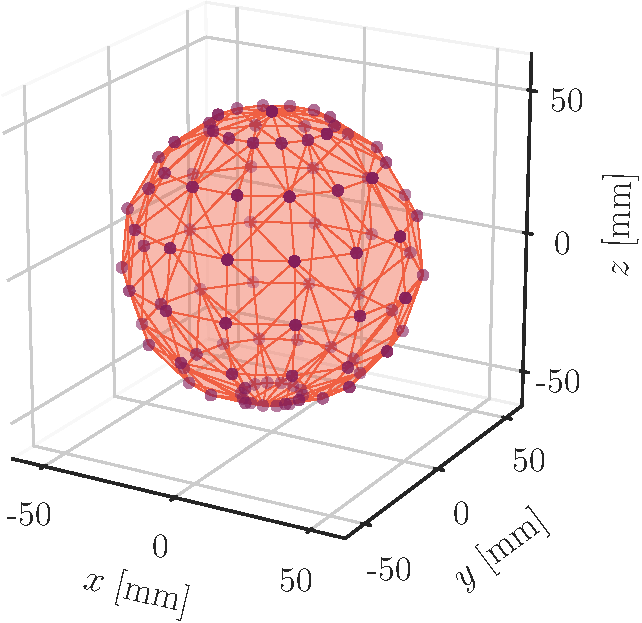
\includegraphics[width=\linewidth]{artwork/spherical_model.pdf}
        \caption{Spherical model.}
        \label{fig:spherical_model}
    \end{subfigure}
    \hfil
    \begin{subfigure}[b]{0.47\textwidth}
        \centering
        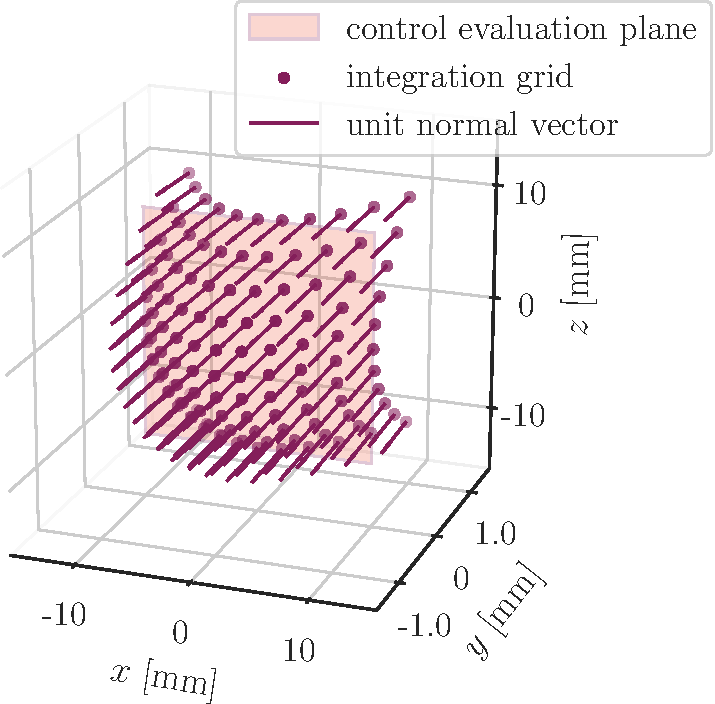
\includegraphics[width=\linewidth]{artwork/spherical_surface.pdf}
        \caption{Spherical averaging surface.}
        \label{fig:spherical_surface}
        \end{subfigure}
    
    \caption{Spherical model with radius set to \SI{5}{\cm}. Spherical averaging surface of \SI{4}{\cm\squared} is represented with integration points that serve as an origin to unit vector field distributed across that surface.}
    \label{fig:sphere}
\end{figure}
\begin{figure}[ht]
    \centering
    \begin{subfigure}[b]{0.42\textwidth}
        \centering
        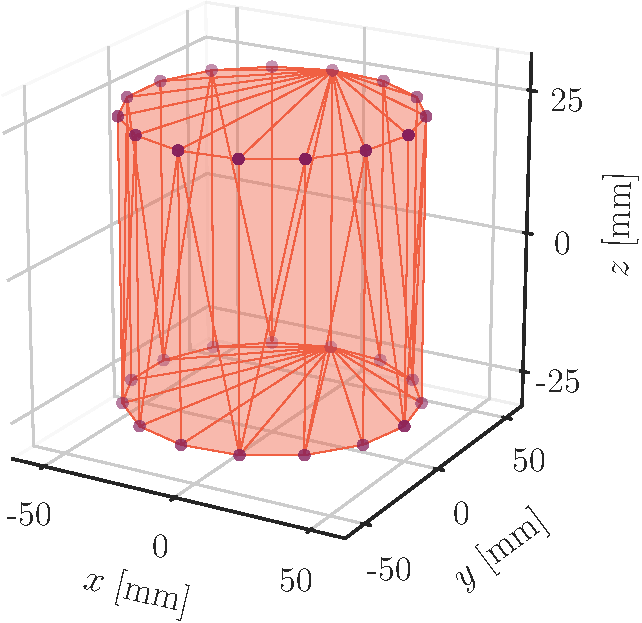
\includegraphics[width=\linewidth]{artwork/cylindrical_model.pdf}
        \caption{Cylindrical model.}
        \label{fig:cylindrical_model}
    \end{subfigure}
    \hfil
    \begin{subfigure}[b]{0.47\textwidth}
        \centering
        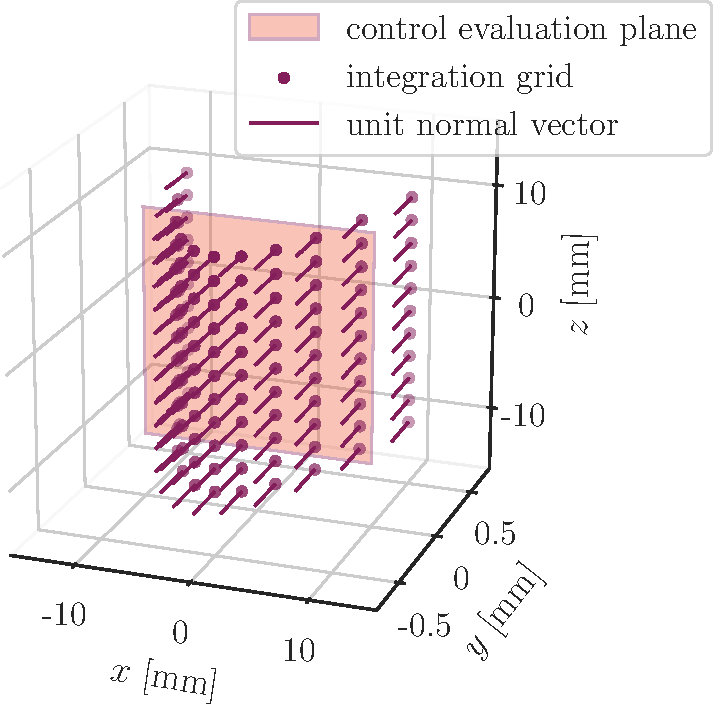
\includegraphics[width=\linewidth]{artwork/cylindrical_surface.pdf}
        \caption{Cylindrical averaging surface.}
        \label{fig:cylindrical_surface}
        \end{subfigure}
    
    \caption{Cylindrical model with radius and height both set to \SI{5}{\cm}. Cylindrical averaging surface of \SI{4}{\cm\squared} is represented with integration points that serve as an origin to unit vector field distributed across that surface.}
    \label{fig:cylinder}
\end{figure}

Some of the proposed averaging techniques, which are currently being discussed within a working group 7 under Subcommittee 6 of \gls{ieee} International Committee on Electromagnetic Safety Technical Committee 95, are directly motivated by the schemes proposed in~\cite{Diao2020Assessment}.
In this work, the assessment of the \gls{apd} on non-planar canonical surfaces at the \SIrange[range-units=single,range-phrase=--]{6}{60}{\GHz} range for a realistic forearm model~\cite{Diao2020Assessment} have been proposed.
Given the body parts are represented as the voxelized models, authors have adopted the definition of the \gls{apd} as given in \cref{eqn:apd_1} for practical reasons and for ease of computation.
Four distinct schemes for the spatial averaging of the \gls{apd} have been presented and are shown in \cref{fig:diao2020assessment}.
The definition of the integration volumes for different schemes are bounded by red polygons as follows.
The upper bound, L1, is parallel to the grid axis in \cref{fig:diao2020assessment}(a) and \cref{fig:diao2020assessment}(b) to match the standard evaluation plane commonly encountered in literature.
On the other hand, the upper bound, L1, is bent along the surface to approximately match the curvature of skin in \cref{fig:diao2020assessment}(c) and \cref{fig:diao2020assessment}(d).
Side bounds, L2 and L3, are parallel to the grid axis in \cref{fig:diao2020assessment}(a) and \cref{fig:diao2020assessment}(c),  whereas in \cref{fig:diao2020assessment}(b) and \cref{fig:diao2020assessment}(d), L2 and L3 are parallel to the internal electric field gradients at the model surface.
In all schemes, the lower bound, L4, is defined as the contour where the electric field is at $1/1000$ of the maximum value in the integration volume.
\begin{figure}[ht]
    \centering
    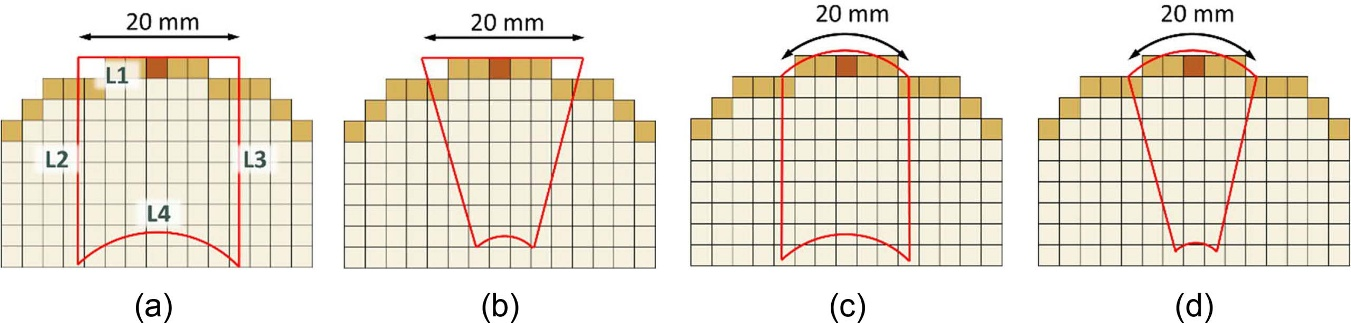
\includegraphics[width=\textwidth]{artwork/Diao2020Assessment_figure2.png}
    \caption{Figure 2. in~\cite{Diao2020Assessment}: ``Definitions of the integration volumes for the different absorbed power density calculation schemes. (a) Scheme 1, (b) Scheme 2, (c) Scheme 3, and (d) Scheme 4.''}
    \label{fig:diao2020assessment}
\end{figure}
As these types of voxelized representations of the human body are known to suffer from stair-casing numerical errors~\cite{Poljak2018On}, a novel local compensation method has been established which allows for correcting the heat convection rate and is validated by the analytical solution by using a simple spherical model and prolate ellipsoidal models. 
Overall, authors conclude that for the model curvature radius $> \SI{30}{\mm}$ at and above \SI{20}{\GHz}, the heating factors agree well with those obtained in previous studies using planar models, and the differences in the heating factors among different proposed schemes for assessment of the spatially-averaged \gls{apd} on non-planar surfaces are marginal.

\Gls{em} exposure assessment of the \gls{ipd} on spherical head model up to \SI{100}{\GHz} is provided in~\cite{Kapetanovic2022AssessmentTEMC}.
In this study, the radiating source was modelled as the half-wavelength dipole antenna placed in close proximity of the spherical model with radius corresponding to that of the average human male.
It has been shown that the spatial averaging of the incident power density at the \SIrange[range-units=single,range-phrase=--]{3.5}{100}{\GHz} range yields to up to \SI{30}{\percent} greater values compared to the common planar surface.
Interestingly, authors positioned the evaluation plane at three distinct locations with respect to the spherical averaging surface which closely resembles the one shown in \cref{fig:spherical_surface}.
Namely, the first planar averaging surface corresponding to the worst case exposure scenario is placed onto a tangential plane of the nearest point on the spherical averaging surface.
The second planar averaging surface is located on a plane intersecting the spherical averaging surface at 4 points in the middle – between the nearest point and 4 farthest points on the surface of the spherical averaging surface relative to the antenna position.
Finally, the last considered planar averaging surface intersects the spherical averaging surface at 4 farthest points relative to the antenna position.
Two definitions of the \gls{ipd} as presented in~\cite{IEEE2021Guide} are used for the \gls{em} analysis and are adjusted to the spherical coordinate system to enable to allow the use of 2-D numerical integration over the parameterized averaging surface.
The 2-D Gauss-Legendre quadrature is used to define a suitable choice of integration nodes across this parameterized surface. Surface integrals is then approximated as a sum of incremental contributions across the parametric surface at integration nodes (see \cref{fig:spherical_surface}), scaled with proper weights derived at each corresponding node.

Furthermore, in a very recent work~\cite{Taguchi2022Computation}, the \gls{apd} is assessed in high-resolution head models by varying structural parameters, e.g., the skin thickness and smoothness of the surface, above \SI{6}{\GHz}.
The procedure of the assessment of the spatial maximum \gls{apd} on voxelized human head model by using the expression given in \cref{eqn:apd_1} is as follows.
The \gls{apd} value of each surface voxel is projected onto a plane perpendicular to the direction of the impinging wave.
Then, the averaging of the values obtained in the first step is performed over \SI{4}{} or \SI{1}{\cm\squared}, depending on the frequency, with the projected voxel as the center.
The spatial maximum value from the previous step is defined as the relevant \gls{apd}.
It is found that \gls{apd} is below the threshold prescribed by exposure limits in all cases except at \SI{6}{GHz} where the dipole antenna is placed at the separation distance of \SI{45}{\mm} from the pinna.
Authors hypothesize that this discrepancy occurs because of the power absorption being concentrated around the pinna owing to its complex morphology.
Instead of the actual surface area (which can be significantly larger than planar projections in case of emphasized curvature), the normalization in this study is performed by using the parametric projection fixed to \SI{4}{} or \SI{1}{\cm\squared} which can be the main reason of this overestimation.
Authors argue that this approach leads to more conservative dosimetric predictions and thus preferred.
Overall, the results of this study suggest that the effect of varying parameters is marginal in the realistic range.

In~\cite{Kapetanovic2022AssessmentJERM}, the problem of estimation of dosimetric quantities on non-planar body parts is addressed by developing a novel strategy for the assessment of the \gls{apd} on the anatomical model of the human ear.
Considering that the model is morphologically accurate and defined by using the 3-D point cloud rather than by using voxels, the estimation of the unit vector field normal to the surface of the model itself -- which is a key step during surface integration, is the greatest contribution of this study.
The proposed method in this work does not require constructed positional connections between points in 3-D space in which the absorbed \gls{em} field is assessed.
Reconstruction of the surface is performed functionally by enforcing 3-D radial basis function interpolation and, at each point on the averaging surface, the normal vector is estimated by using the principal component analysis.
Details are omitted for the sake of brevity, but are available in the appendix of this study.
The dosimetric analysis is performed in similar manner as in~\cite{Taguchi2022Computation} where only the maximum value of the \gls{apd} for the plane-wave exposure at \SI{26}{} and \SI{60}{\GHz} is reported.
Contrary to~\cite{Taguchi2022Computation}, the normalization of the averaged power density is not performed by using the fixed parametric surface area (black empty square in \cref{fig:kapetanovic2022assessment}) of either \SI{4}{} or \SI{1}{\cm\squared}, rather the actual conformal surface area (red full square in \cref{fig:kapetanovic2022assessment}) is used.
The conformal area is defined by projecting the contours of this parametric surface onto the surface of the ear to mark the region where the power density distribution is computed.
As the conformal surface is not planar, the overall area is at least equal (for a perfectly planar interface) and generally larger than the area of the corresponding parametric surface.
The accuracy of the proposed method and obtained results is verified with established commercial \gls{em} software.
Additionally, numerical comparison of the two definitions of \gls{apd} (see \cref{eqn:apd_1,eqn:apd_2}) is provided.
\begin{figure}[ht]
    \centering
    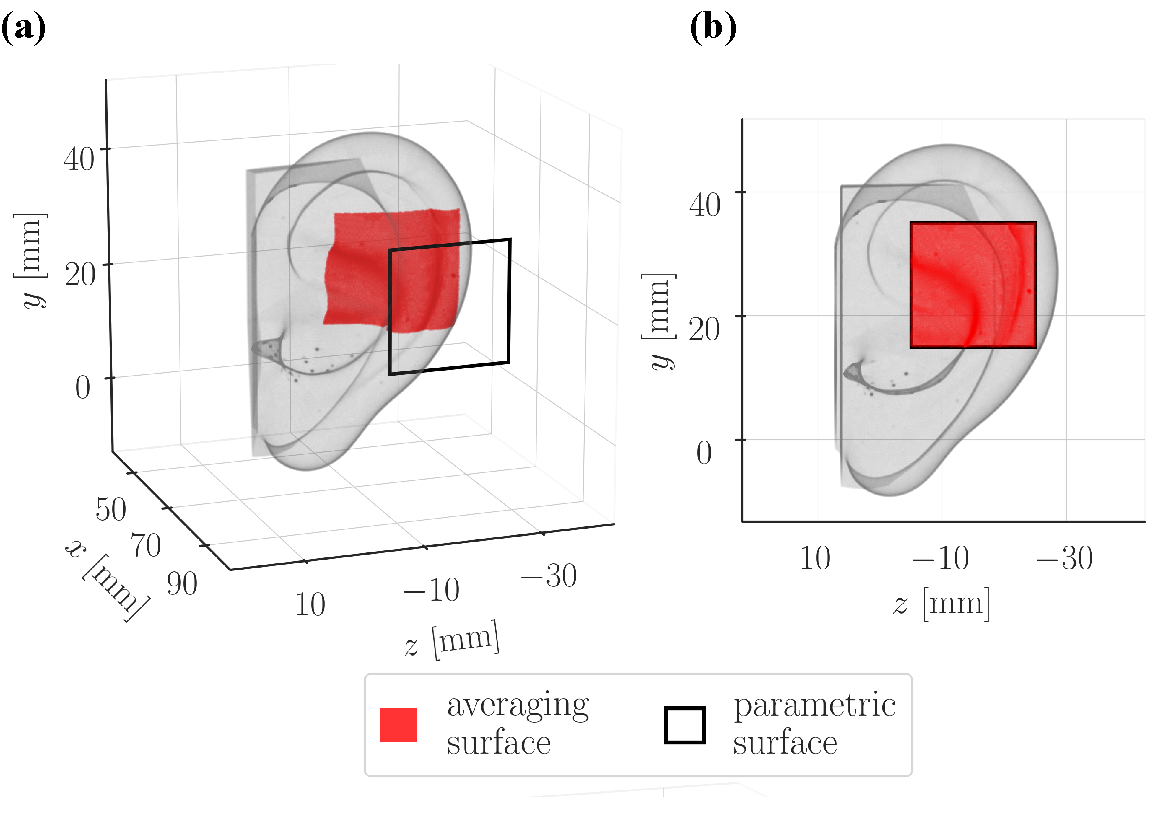
\includegraphics[width=0.8\textwidth]{artwork/Kapetanovic2022Assessment_figure2.pdf}
    \caption{Figure 2. in~\cite{Kapetanovic2022AssessmentJERM}: ``Conformal surface and its corresponding 2-D parametric projection of \SI{4}{\cm\squared} area. (a) 3-D view, and (b) The plane-wave incidence point of view.''}
    \label{fig:kapetanovic2022assessment}
\end{figure}
The results suggest that only a marginal difference between the values obtained from the two different definitions (within about \SI{6}{\percent}) is present regardless of the exposure scenarios.
However, by comparing the same results with common flat tissue-equivalent models, the spatial maximum \gls{apd} on the ear is up to about \SI{20}{\percent} larger regardless of definition.

In~\cite{Morimoto2022Assessment}, the effect of two distinct averaging shapes of the evaluation of the \gls{apd} and \gls{ipd} is investigated computationally.
The main goal of this study is to bridge the existing gap between exposure and product standards.
Namely, in two current international exposure limits, i.e., \gls{icnirp} guidelines~\cite{ICNIRP2020Guidelines} and the \gls{ieee} standard~\cite{IEEE2019Standard}, the averaging area for the assessment of the \gls{apd} and corresponding \gls{ipd} is square shaped and set to \SI{4}{\cm\squared} at the \SIrange[range-units=single,range-phrase=--]{6}{300}{\GHz} range.
Additionally, above \SI{30}{\GHz}, a square-shaped averaging area of \SI{1}{\cm\squared} should be considered as well to account for the small beam formation at the exposed surface.
On the other hand, international standards for product assessment~\cite{IEC2018,IEC2022part1,IEC2022part2} prescribe an averaging scheme of a circular shape in case of non-planar exposed surface for both computational and experimental evaluation of the \gls{ipd} to account the uncertainty during the assessment.
For this inconsistency, authors argue that it is of utmost importance to appropriately define the shape of the averaging surface following the exposure standard rather than product standard as the latter is based on the limits prescribed in exposure standards.
Furthermore, in the \gls{icnirp} guidelines on limits of exposure to laser radiation~\cite{ICNIRP2013Guidelines} that pertains to frequencies above \SI{300}{\GHz}, it is also a circular shape that is suggested as probe aperture for measurements of the power density at the surface of exposed tissue.
For this reason also, authors argue again that the discontinuation of the use of the averaging shape is of special interest.
In this study, planar homogeneous tissue-equivalent models and the human anatomical model are used to assess compliance and compute the the difference in the spatially averaged dosimetric quantities between square and circular averaging shapes by means of the heating factor.
Both models are irradiated by using dipole antennas and dipole arrays in various configuration at different distances.
The maximum differences in heating factors of the \gls{apd} and \gls{ipd} for square and circular averaging areas are marginal (in both cases about \SI{4}{\percent}) at the antenna-to-tissue separation distance $> \SI{5}{\mm}$ and are pronounced mostly when the surface of the model is elliptical in shape.
Overall, the heating factors for both the \gls{apd} and \gls{ipd} averaged on a circular averaging shape are conservative in comparison to those obtained for a square averaging shape up to \SI{300}{\GHz}.
The only exception is then the incident angle of the beam is within the \SIrange[range-units=single,range-phrase=--]{30}{60}{\degree} range.

This subject is further explored in a small scale study in~\cite{Kapetanovic2022Assessment} where the assessment of the spatially-averaged \gls{apd} on a realistic ear model is provided.
The \gls{em} analysis is performed computationally for plane wave exposure at \SI{60}{\GHz}.
The effect of the averaging area shape by using the same shape types, i.e., the square and disk both with the area of \SI{1}{\cm\squared}, as in~\cite{Morimoto2022Assessment} on the \gls{apd} is investigated.
By comparing the values of the \gls{apd} with different polarization of the impinging plane wave, a substantial relative difference of \SI{14}{\percent} between transverse electric and magnetic polarization is present on a circular averaging area.
On the other hand, negligible differences (up to \SI{2}{\percent}) exist between the \gls{apd} on different averaging area shape.
Authors conclude that, according to the studied exposure scenarios, variations in \gls{apd} as a function of the averaging surface shape are less significant than those related to the electric characteristics of the incident field.